

\chapter{Dereverberation based on RIR constrained cost function}
\label{chapter:icassp2017}

This chapter explains NMF based dereverberation methods that utilize three different properties of RIR spectrogram - sparsity, frequency envelope, and early part of RIR. Such methods are derived by modifying the basic NMF based dereverberation methods available in the literature. The initial section of this chapter explains the basic NMF based dereverberation problems. Later part of the chapter explains the modifications made to accommodate the above mentioned RIR properties in the dereverberation problem. This discussion is followed by the analysis of enhancement results. 

\section{Basic NMF based dereverberation methods}
\label{sec:basic_NMF_reverb_model}
This section explains the approach taken to estimate clean speech and RIR spectrogram based on the basic reverberation models discussed in Section~\ref{sec:NMF_methods}. The algorithms based on the CNMF reverberation model in (\ref{eq:cnmf0}) and CNMF reverberation model with NMF clean speech model in (\ref{eq:cnmf1}) is discussed next. 

\subsection{CNMF based reverberation model}
The CNMF model for reverberated speech spectrogram was discussed in Section~\ref{sec:NMF_methods}. In~(\ref{eq:cnmf0}), the reverberated speech spectrogram $Y_R\in\mathbb{R}_+^{K \times T}$ is approximated as convolution of clean speech spectrogram $\mathbf{S}\in\mathbb{R}_+^{K \times (T-L_h+1)}$ and RIR spectrogram $\mathbf{H}\in\mathbb{R}_+^{K \times L_h}$. 
\begin{equation}
Y_R(k,n)\approx \sum_{l=0}^{L_h-1} H(k,l)S(k,n-l),
\label{eq:cnmf0_1}
\end{equation}
where $Y_R(k,n)\text{, } H(k,n) \text{ and }S(k,n)$ represents the elements of $\mathbf{Y_R}\text{, } \mathbf{H} \text{ and }\mathbf{S}$, respectively.
Iterating algorithm was proposed for solving for $S(k,n)$ and $H(k,n)$ based on reverberation model in (\ref{eq:cnmf0_1})~\cite{kameoka2009robust,Kumar2011}. The parameters are estimated such that it minimizes a cost function. Euclidean distance (ED)~\cite{kameoka2009robust} and generalized KL divergence~\cite{Kumar2011} are commonly used cost functions. Generalized KL divergence (KL) as cost functions gives reduced modeling error when compared to ED. The optimization problem for solving the CNMF based reverberation model based on KL divergence can be written as,
\begin{align}
&C_{cnmf0} = \underset{S(k,n)\text{, }H(k,n)}{\text{argmin}} \Bigg[ \sum_{k,n} \text{KL} \bigg(Y_R(k,n)|\tilde{Y}_R(k,n)\bigg)+\lambda_{cnmf0}\sum_{k,n}S(k,n) \Bigg] \nonumber \\ 
\text{Subjected to}& \nonumber \\
&H(k,n) \geq 0\text{, }S(k,n)\geq 0 \nonumber \\ 
&\sum_{n}H(k,n) = 1 \text{,}
\label{eq:cost_cnmf0}
\end{align}
where $\tilde{Y}_R(k,n)$ represents the estimated reverberated spectrogram based on (\ref{eq:cnmf0_1}). $\lambda_{cnmf0}$ is a weighting factor. The cost function in (\ref{eq:cost_cnmf0}) has two terms. First term is a measure of deviation between actual and estimated reverberated speech spectrogram. The second term introduces sparsity to the estimated clean speech spectogram. The amount of sparsity is controled by $\lambda_{cnmf0}$. It is fixed as $\lambda_{cnmf0}=\dfrac{10^{-8}}{KT}\sum\limits_{k,n}Y_R(k,n)$. This first set of constraints make sure that the estimated $S(k,n)$ and $H(k,n)$ are non-negative. This is necessary as these terms represents magnitude spectrograms. The normalization $\sum\limits_{n}H(k,n) = 1$ was required to avoid scaling ambiguity and the subsequent estimation of undesired solution~\footnote{Assume a clean speech spectrogram $S(k,n)$ and RIR $H(k,n)$ minimizes the first term in (\ref{eq:cnmf0_1}). Then $aS(k,n)\text{, }a\in \mathbb{R}_+$ and $H(k,n)/a$ will also minimizes the first term. So, the cost function (\ref{eq:cnmf0_1}) is minimized by the value that minimizes the second term. This happens when $S(k,n)=0$, resulting in $H(k,n)=\infty$.}. Iterative algorithm based on a multiplicative update rule was proposed to find the solution~\cite{Kumar2011}. The update rule for the parameters are shown in (\ref{eq:multi_update_cnmf0}). This method is referred to as CNMF0.
\begin{align}
H(k,n) & \leftarrow H(k,n) \dfrac{\sum\limits_l\dfrac{Y_R(k,l)}{\tilde{Y}_R(k,l)}S(k,n-l)}{\sum\limits_l S(k,n-l) } \nonumber \\
S(k,n) & \leftarrow S(k,n)\dfrac{\sum\limits_l\dfrac{Y_R(k,l)}{\tilde{Y}_R(k,l)}H(k,n-l)}{\sum\limits_l H(k,n-l) + \lambda_{cnmf0}} 
\label{eq:multi_update_cnmf0}
\end{align}

The steps involved in CNMF0 is summarized in Algorithm~\ref{algo:cnmf0}. The time-domain de-reverberated speech is obtained by performing an inverse STFT on the complex spectrogram of the estimated clean speech. The complex spectrogram is constructed by using the phase spectrogram obtained from the reverberated speech along with the enhanced magnitude spectrogram.  
% spectrogram comparison plots

%\iffalse
\begin{algorithm}[H]
\SetAlgoLined
\KwResult{ Enhanced speech spectrogram $S(k,n)$ }
 initialize $S(k,n)$, $H(k,n)$ to random positive values\;
  \For{$i=1:\text{i\_max}$}{
    update $S(k,n)$\\
    update $H(k,n)$\\
    normalization $H(k,n) \leftarrow \dfrac{H(k,n)}{\sum\limits_n H(k,n)}$
    }
 \caption{Steps involved in CNMF0}
 \label{algo:cnmf0}
\end{algorithm}
%\fi
\subsection{CNMF model with NMF model for clean speech}
The CNMF reverberation model was modified by incorporating a model for clean speech. The clean speech spectrogram was approximated using a NMF model as, 
\begin{align}
\mathbf{S}&\approx \mathbf{W}_s\mathbf{X}_s \nonumber \\
S(k,n)&\approx \sum\limits_{r=1}^{R_s} W_s(k,r)X_s(r,n),
\end{align}
where $\mathbf{W}_s\in\mathbb{R}_+^{K\times R_s}$ and $\mathbf{X}_s\in\mathbb{R}_+^{R_s\times (T-L_h+1)}$ represents the bases and activation matrix. $R_s$ represents the rank of NMF decomposition. $W_s(k,r)$ and $X_s(r,n)$ are elements of $\mathbf{W}_s$ and $\mathbf{X}_s$, respectively. Utilizing the NMF model in (\ref{eq:cnmf0_1}), the reverberation model can be rewritten as,
\begin{equation}
Y_R(k,n)\approx \sum\limits_{l=0}^{L_h} H(k,l)\bigg[\sum\limits_{r=1}^{R_s}W_s(k,r)X_s(r,n-l)\bigg]
\label{eq:cnmf1_1}
\end{equation}
An algorithm was proposed to obtain clean speech and RIR spectrograms from reverberation model in (\ref{eq:cnmf1_1})~\cite{mohammadiha2016speech, Mohammadiha2015}. The optimization problem can be summarized as,
\begin{align}
&C_{cnmf1} = \underset{\mathbf{H}\text{, }\mathbf{W}_s\text{, }\mathbf{X}_s}{\text{argmin}} \Bigg[ \sum_{k,n} \text{KL} \bigg(Y_R(k,n)|\tilde{Y}_R(k,n)\bigg)+\lambda_{cnmf1}\sum_{r,n}X_s(r,n) \Bigg] \nonumber \\ 
\text{Subjected to}& \nonumber \\
&H(k,n) \geq 0\text{, }W_s(k,r)\geq 0\text{, }X_s(r,n)\geq 0 \nonumber \\ 
&H(k,0) = 1\forall k\in \{0,1,...,(K-1)\} \text{,}
\label{eq:cost_cnmf1}
\end{align}
where $\tilde{Y}_R(k,n)$ represents the estimated reverberated spectrogram based on reverberation model in (\ref{eq:cnmf1_1}). $\lambda_{cnmf1}$ represents a weighting factor. The objective function has two terms. The first term minimizes the modeling error between estimated and actual reverberated speech spectrograms. The second term introduces sparsity in estimated clean speech activation. The first set of constraints ensures that the estimated clean speech and RIR spectrograms are non-negative. Normalization in the RIR spectrogram removes the inherent scaling ambiguity present in the cost function.

Multiplicative update rule was obtained for solving the optimization problem in (\ref{eq:cost_cnmf1})~\cite{mohammadiha2016speech, Mohammadiha2015}. The update rules are summarized in (\ref{eq:multi_update_cnmf1}).
\begin{align}
H(k,n) & \leftarrow H(k,n) \dfrac{\sum\limits_l\dfrac{Y_R(k,l)}{\tilde{Y}_R(k,l)}S(k,n-l)}{\sum\limits_l S(k,n-l) } \nonumber \\
W_s(k,r) & \leftarrow W_s(k,r) \dfrac{\sum\limits_{n,l}\dfrac{Y_R(k,n)}{\tilde{Y}_R(k,n)} H(k,l)X_s(r,n-l)}{\sum\limits_{n,l} H(k,l)X_s(r,n-l)} \nonumber \\
X_s(r,n) & \leftarrow X_s(k,r) \dfrac{\sum\limits_{k,l}\dfrac{Y_R(k,l)}{\tilde{Y}_R(k,l)} H(k,n-l)W_s(k,r)}{\sum\limits_{k,l} H(k,n-l)W_s(k,r)+\lambda_{cnmf1}}
\label{eq:multi_update_cnmf1}
\end{align}
where $\tilde{S}(k,n)=\sum\limits_r W_s(k,r)X_s(r,n)$.
There exists two approaches. This distinction is based on how $W_s(k,r)$ is estimated. In unsupervised (offline) approach, the clean speech bases $W_s(k,r)$ is estimated from the reverberated data. This approach is referred to as \text{CNMF1\_u}. In supervised (online) approach, $W_s(k,r)$ are pre-learned. A NMF decomposition is performed on the spectrogram of available clean speech recording. The bases vectors obtained for this decomposition forms $W_s(k,r)$. This method is referred to as \text{CNMF\_s}. The steps involved are summarized in Algorithm~\ref{algo:cnmf1}. 

\begin{algorithm}[H]
\SetAlgoLined
\KwResult{ Enhanced speech spectrogram $S(k,n)$ }
 initialize $W_s(k,r)$, $X_s(r,n)$, $H(k,n)$ to random positive values\;
  \For{$i=1:\text{i\_max}$}{
     \If{$W_s(k,r)$ is not fixed}{
      update $W_s(k,r)$\\
      }
    update $X_s(r,n)$\\
    update $H(k,n)$\\
     \If{$H(k,n)>H(k,n-1)$}{
      truncation of $H(k,n)$ \\ 
      $H(k,n)\leftarrow \text{min}\bigg( H(k,n), H(k,n-1) \bigg)$\\
      }    
    normalization $H(k,n) \leftarrow \dfrac{H(k,n)}{ H(k,0)}$
    }
  estimation of clean speech spectrogram 
  $S(k,n)=\dfrac{\sum\limits_{r=1}^{R_s} W_s(k,r)X_s(r,n)}{\tilde{Y}_R(k,n)}Y_R(k,n)$
 \caption{Steps involved in \text{CNMF1\_s and CNMF1\_u} }
 \label{algo:cnmf1}
\end{algorithm}

\subsection{Comparison of reverberation models}

\section{Incorporation of RIR properties on optimization problem}
The NMF based dereverberation methods discussed in Section~\ref{sec:basic_NMF_reverb_model} used properties of clean speech spectrogram like low-rank nature and sparsity. However, such methods did not incorporate any properties of RIR except for basic truncation and normalization of the RIR spectrogram. This chapter focuses on incorporating three meaningful constraints on the RIR spectrogram to improve the dereverberation performance of basic NMF based dereverberation methods. The properties of RIR used are (i) frequency envelope of RIR spectrogram, (ii) sparsity of RIR spectrogram, and (iii) retaining the early part of the RIR spectrogram. These approaches are explained in detail next.

\subsection{Frequency envelope of RIR spectrogram}
\subsection{Sparsity of RIR spectrogram}
\subsection{Retaining early part of RIR}

\iffalse
\section{Requirement}
\begin{itemize}
\item NMF based reverberation methods does not use RIR model (except truncation) in cost function
\item Also does normalization on RIR spectrogram 
\item Resulting in sub-optimal performance
\end{itemize}
\section{Proposed approach}
\begin{itemize}
\item introduces constraints on estimated RIR spectrogram in cost function
\item incorporate both speech and RIR model
\item improving speech enhancement results and proper RIR estimates
\item Three appraoches
\begin{itemize}
\item frequency envelope of RIR
\item sparsity on RIR spectrogram
\item retaining early part of RIR
\end{itemize}  
\end{itemize}
\section{Experimental results - enhancement results} 
\section{Discussions} 
\fi

\iffalse
Distant speech enhancement and recognition has been gaining importance over the
past decade due to the prevalence of audio capturing
instruments~\cite{Kumatani2012}. Such
instruments could be mobile phones, voice recorders, microphones in a conference
room or an automobile. Distant speech refers to scenarios where the audio source
and capturing device are separated at least by a feet. Speech processing (for
recognition or enhancement) in such environments differs from traditional speech
processing as it has to compensate for reverberation effects in the captured
data. While speech dereverberation has been an active research area for a long
time~\cite{naylor2010speech}, it has gained interest recently~\cite{reverb2014}
for the reason mentioned above. Speech dereverberation can be done using single-
or multi-channel data depending on the application of interest. The main objective in
this research is to address single-channel dereverberation in the distant speech scenario. The performance is evaluated for both speech enhancement and automatic speech recognition task. 

The effect of reverberation on speech depends not only on the speech signal, but
also on the room or environment under consideration. Reverberation alters speech
in a way much different from other types of environmental noise. The environment
or the room can be modelled as an impulse response or specifically as room
impulse response (RIR). The characteristics of this RIR have a significant
effect on the reverberant signal, and hence a good understanding of this is
relevant for dereverberation. This is more important when addressing this
problem as a blind deconvolution problem. 

Dereverberation methods can be classified as those that (i) cancel reverberation or
(ii) suppress reverberation. The reverberation cancellation methods include blind
deconvolution based methods. The reveberation suppression methods include
spectral substraction, linear prediction (LP) based methods, and statistical
methods for spectral enhancement. Here we consider a non-negative matrix
factorization (NMF) based approach that can be classified as reverberation suppression
approach. This uses the magnitude spectrum of the reverberant signal, and with
minimal prior knowledge of the RIR, to obtain the dereveberated speech signal.
The earliest work to introduce the notion of NMF for
dereverberation~\cite{kameoka2009robust} provides a statistical motivation for use of NMF
to solve the dereverberation problem. More recently there have been several
improvements over the basic NMF based approache for dereverberation in both
single-channel~\cite{Mohammadiha2016, baby2016supervised, Mohammadiha2015, Kallasjoki2014, Kumar2011}, and multi-channel~\cite{Yu2012}, ~\cite{Yu2014}, ~\cite{Mirsamadi2014} scenarios.
In~\cite{Mohammadiha2016, Mohammadiha2015} the initial NMD model for speech
dereverberation is improved by integrating various NMF models for the speech
signal within the original model leading to several NMD-NMF approaches. The work
in~\cite{baby2016supervised} along with a NMD-NMF approach uses a NMF model for external
additive noise and hence does both dereverberation and denoising. Most of
these methods use the short-time Fourier transform (STFT) spectrum representation of the
signal when performing NMF. The method proposed in~\cite{Kumar2011} uses a
gammatone filtered spectrum in the NMF framework and has shown improvements in
word error rates (WER) over the earlier NMF based methods. These methods also
have proposed incorporating a sparsity constraint on the speech signal as a
regularizer to improve speech enhancement. All these approaches
have demonstrated improvement in speech enhancement measures
and or WER improvement. NMF based methods for dereverberation provide an
estimate of the clean speech signal and the corresponding room impulse response
(RIR). While the estimation accuracy of the speech signal is considered in all
existing approaches, they do not provide an evaluation of the accuracy of the
RIR estimate. The single-channel NMF dereverberation problem is treated as a
deconvolution in the sub-band domain. Obtaining the RIR from the observed
reverberant signal is a unconstrained problem and possibly many solutions.
Hence, its required to impose appropriate constraints in obtaining the solution.
Earlier NMF approaches obtained reasonable estimates for speech by imposing a
sparsity constraint or by using appropriate models for speech. The objective in
this work is to consider the RIR estimates and relate them to the expected
estimates, within the reverberation model constraints. Such an analysis is used
further to provide regularizations or constraints on the RIR, leading to better
estimates of both the clean speech signal and RIR of the system. These
constraints are motivated from both time-domain and frequency-domain models of
the revereberant RIR~\cite{naylor2010speech}. The proposed regularization on RIR
will be evaluated using speech enhancement measures such as PESQ, SRMR, and CD. The speech enhancement task is evaluated using improvement in WER.
%These guidelines include complete descriptions of the fonts, spacing, and
%related information for producing your proceedings manuscripts. Please follow
%them and if you have any questions, direct them to Conference Management
%Services, Inc.: Phone +1-979-846-6800 or email
%to \\\texttt{papers@ieee-icassp2017.org}.

\section{NMF based speech dereverberation}
The reverberant speech model considered when using NMF for dereverberation and a
brief description of existing NMF approaches to solve this problem are described
in this section. The goal of NMF algorithms is to factorize a non-negative
matrix $\mat{V} \in \mathbb{R}^{F \times T}$, consisting of elements $v_{i,j} >
0, \forall i,j$, into a product of two non-negative matrices $\mat{W} \in
\mathbb{R}^{F \times R}$ and
$\mat{U} \in \mathbb{R}^{R \times T}$, such that
\begin{equation}
\mat{V} = \mat{W} \mat{U}.
\label{eqn:NMFBasicProduct}
\end{equation}
Here, the columns $w_i\in \mathbb{R}^{F \times 1}, i \in \{1,\ldots, R\}$ of $\mat{W}$ can be considered as a set
of basis vectors and the rows $u_i\in\mathbb{R}^{1 \times T}, i \in \{1, \dots, R\}$ of $\mat{U}$ are the
weights or activations to obtain the columns $v_i, i \in \{1, \ldots, T\}$ of
$\mat{V}$. Efficient algorithms to solve (\ref{eqn:NMFBasicProduct}) using
multiplicative-updates were initially proposed in~\cite{lee99}. Since then NMF
algorithms have been used in several applications. In speech or audio
processing, NMF can be applied if the magnitude spectrum of the signal is
considered as $\mat{V}$. Several variants of NMF have been proposed for source
separation, denoising, and enhancement of speech and music signals. Here, we will restrict our discussion to the use of NMF for speech
enhancement or dereverberation.    

% reverberant speech model
For NMF to be used in speech dereverberation the spectral representation of the
observed or reverberated signal needs to be understood. In time-domain, the observed signal
$x[n]$ in a microphone as result of a clean speech signal $s[n]$ in a
reverberant room with room impulse response (RIR) $h[n]$, can be represented as
\begin{equation}
  x[n] = s[n] * h[n] = \sum_{m=0}^{M-1} h[m] s[n-m],
  \label{eqn:reverb_t}
\end{equation}
where $*$ represents convolution in time-domain, and $M$ is the length
of the RIR. In NMF we require a frequency-domain representation of the signal.
Hence, we are interested either in the short-time Fourier transform (STFT)
representation or any equivalent transform where a representation as
in~(\ref{eqn:NMFBasicProduct}) is possible. Here, we will consider the magnitude of
the STFT spectrum of the signal and follow a representation motivated
in~\cite{kameoka2009robust} and later followed
in~\cite{Kumar2011},~\cite{Mohammadiha2016}.  
One main aspect of this representation is that it handles the reverberant RIRs
which are typically longer (in 100s of ms) compared to the STFT analysis window
duration of 20-40~ms considered in speech analysis. In this STFT model, the STFT
of the reverberated signal is considered as a convolution of the $s[n]$ and
$h[n]$ in each of the sub-bands~\cite{Yekutiel2007}, \cite{kameoka2009robust} i.e.,
\begin{equation}
  x[k,n] \approx \sum_{m=0}^{L_h-1} h[k, m] s[k, n-m],\ k\in\{0,1,...,K-1\}
  \label{eqn:reverb_k}
\end{equation}
where $x[k,m]$, $h[k,m]$, $s[k,m]$ are the STFT representation of reverberated
signal, RIR, and clean speech signal, respectively, $L_h$ is the length of RIR
in the STFT domain, and $K$ is the number of frequency bands in the STFT
representation. With this underlying model, it has been observed
in~\cite{Kumar2011},~\cite{Mohammadiha2016} that a similar representation can be
obtained when using the magnitude of the STFT coefficients. i.e.,
\begin{equation}
  |x[k,n]| \approx \sum_{m=0}^{L_h-1} |h[k, m]| |s[k, n-m]|, k\in\{0,1,...,K-1\}.
  \label{eqn:reverb_k_mag}
\end{equation}
For ease of notation, we drop the $| . |$ and use the following equation to
denote the model that uses the magnitude of STFT spectrum,
\begin{equation}
   X[k,n] \approx \sum_{m=0}^{L_h-1} H[k, m] S[k, n-m], k\in\{0,1,...,K-1\}.
  \label{eqn:reverb_k_matrix}
\end{equation}
To be consistent with~\cite{Mohammadiha2016} we will refer
to~\eqref{eqn:reverb_k_matrix} as the non-negative convolutive transfer function
(N-CTF) model for reverberation.


% NMF approaches for solving dereverberation
The earliest attempt to solve~\eqref{eqn:reverb_k_matrix} using the
non-negativity of the magnitude squared of the spectrum was
in~\cite{kameoka2009robust}. Given the observed sub-band signal $Y[k,m]$
(denotes $|y(k,m)|^2$),
\begin{equation}
  Y[k,n] = X[k,n] + \epsilon[k,n]]
  \label{eqn:robust_cost}
\end{equation}
where $\epsilon$ is considered as the reconstruction error. They obtained a
solution for $S[k,n]$ and $H[k,n]$ to minimize the reconstruction error
assuming it to be Gaussian white noise. In addition to non-negativity
constraints on $S[k,n]$ and $H[k,n]$, they also assumed $\sum_n H[k,n] = 1, \forall k \in \{0,1,...,K\}$ to
avoid indeterminacy in the estimates obtained. They proposed multiplicative
update rules to obtain $S$ and $H$, and also related it to the non-negative
matrix factor deconvolution (NMFD) problem~\cite{Smaragdis2004ConvolutiveNMF}.
The NMFD framework is a variant of the original NMF
formulation in~\eqref{eqn:NMFBasicProduct}, to use a convolutive model as in
\begin{equation}
  \mat{V} \approx \sum_{j=1}^J \mat{W}_j \stackrel{j\rightarrow}{\mat{U}},
  \label{eqn:NMFConvolutive}
\end{equation}
where $\mat{W}$ and $\mat{U}$ are the basis and activation matrices. The
$j\rightarrow$ indicates a column-shift by $j-1$ positions to the right. Using this
NMFD representation, the reverberation model in~\eqref{eqn:reverb_k_matrix} can be represented as
\begin{equation}
  \mat{X} \approx \sum_{m} \mat{H}_m \stackrel{m\rightarrow}{\mat{S}},
  \label{eqn:reverbNMFD}
\end{equation}
where 
\begin{equation}
  \mat{S} = \begin{bmatrix} \mat{s}_1, \mat{s}_2, \ldots, \mat{s}_T
  \end{bmatrix}
  \label{eqn:nmfd_s}
\end{equation}
with $\mat{s}_i \in \mathbb{R}^{K \times 1}, i\in \{1, \ldots, T\}$ and 
\begin{equation}
  \mat{H}_m = \begin{pmatrix} H[1,m] & \ldots & 0 \\ \vdots & \ddots & \vdots \\
    0 & \cdots & H[K,m] \end{pmatrix}.
\end{equation}
a diagonal matrix. As observed in~\cite{kameoka2009robust}, this representation
for the reverberant signal comprises of components of clean speech spectrum are
being blurred by the temporal evolution of the $\mat{H}$ components. With this
the $\mat{H}$ corresponds to a basis matrix constrained to be diagonal and the
clean speech spectrum corresponds to the activation matrix. The solution
proposed in~\cite{mohammadiha2016speech} corresponds to a NMF setting where the
error to be minimized is the Kullback - Leibler (KL) divergence between $\mat{Y}$ and
$\mat{X}$. The general form of the cost-function to be minimized can be represented as
\begin{align}
  J(\mat{S},\mat{H}) &= D_{KL}(\mat{Y}, \mat{X}),\\
  &= D_{KL}(\mat{Y}, \sum_{m} \mat{H}_m \stackrel{m\rightarrow}{\mat{S}}) \\
  \text{s.t.} \sum_m H[k,m] &= 1,\ k\in \{1,\ldots,K-1\},  \mat{H}_m \ge 0, \mat{S} \ge 0.
  \label{eqn:NMFcost}
\end{align}
where $\mat{X}$ is from~(\ref{eqn:NMFConvolutive}) and $D_{KL}(Y \parallel X)$ is defined as follows. 
\begin{equation}
D_{KL}(Y \parallel X)=\sum_{k,m} (Y[k,m]ln(\dfrac{X[k,m]}{Y[k,m]})-X[k,m]+Y[k,m])
\end{equation}
The cost functionin~(\ref{eqn:NMFcost}) is modified to include
sparsity constraint on $\mat{S}$, which leads to better estimates. Improving
on~\cite{kameoka2009robust}, the work in~\cite{Kumar2011} observed that using a
Gammatone filtered magnitude spectrum provides improved estimates compared to
that of using just the Fourier transform. This work also demonstrated the
effectiveness of using the magnitude of the spectrum as opposed to that of
magnitude squared spectrum suggested in~\cite{kameoka2009robust}. The
effectiveness of the NMF algorithm on speech recognition was also demonstrated
here by considering WER measures. In the more recent
work~\cite{Mohammadiha2016}, the NMFD reverberation model was further improved by
incorporating a NMF model for the speech spectrum. The NMF model for the speech
signal has been used in several applications. In matrix notation, the NMF
factorization of the clean speech signal spectrogram can be denoted as
\begin{equation}
  \mat{S} \approx \mat{W} \mat{X}
  \label{eqn:NMFspeech}
\end{equation}
where $\mat{W} \in \mathbb{R}^{F \times R}$ represents a matrix of basis vectors
for clean speech signal and $\mat{X} \in \mathbb{R}^{R \times T}$ is a matrix of
activations. Given the speech spectrogram, the NMF multiplicative updates can be
used to obtain the basis vectors $\mat{W}$ and activations $\mat{X}$.
In~\cite{Mohammadiha2016} such a representation is integrated into the NMFD
model for revereberation, and the corresponding updated cost-function is
\begin{align}
  J(\mat{W}, \mat{X},\mat{H}) &= D_{KL}\left(\mat{Y}, \mat{X}\right),\\
  &= D_{KL}\left(\mat{Y}, \sum_{m} \mat{H}_m
  \stackrel{m\rightarrow}{\mat{S}}\right)\\
  &= D_{KL}\left(\mat{Y}, \sum_m \mat{H}_m \stackrel{m \rightarrow}{\left(\mat{W}
  \mat{X}\right)}\right)
  + \parallel \mat{X} \parallel_1 \\
  \text{s.t.}  \sum_m H[k,m] = 1,& \mat{H}_m \ge 0, \mat{W} \ge 0, \mat{X} \ge 0.
  \label{eqn:NMFD_NMFcost}
\end{align}
where $\parallel \cdot \parallel_1$ denotes $l1$-norm and promotes sparsity.
They also suggested another weighted method that combined the NMFD model for
dereverberation along with the NMF speech model. However, their experiments and
results suggest that the integrated model in~(\ref{eqn:NMFD_NMFcost}) does performs
better and hence not discussed here. The results in~\cite{Mohammadiha2016}
indicate improved speech enhancement measures and do not provide any speech
recognition results. They proposed three possible NMF models for the speech
signal which are either unsupervised or semisupervised. In the unsupervised
method of speech modeling the basis vectors $\mat{W}$ were learnt online from
the reverberant signal and referred to as N-CTF+NMF. The other two methods were
semi-supervised approaches where the basis matrix $\mat{W}$ was learnt offline
from training data. Here they considered two approaches (i) a low-rank NMF model
where $\mat{W}$ was obtained from clean speech training data denoted as
N-CTF+NMF+LR 
(ii) an overcomplete NMF model where the $\mat{W}$ was obtained using a random
walk model to select basis vectors from those obtained using training data denoted as N-CTF+NMF+OC.

In another recent work~\cite{baby2016supervised}, the NMF based approaches
in~\cite{Mohammadiha2016}, ~\cite{kameoka2009robust} have been extended to do both
dereverberation and denoising in a supervised setting. They introduce a NMF model to handle other
background noises, which does not include reverberation, and NMF model for the
speech signal. They learn basis matrices for both speech signal and noise signal
from training data. They demonstrate improvement in speech enhancement measures
using NMF models for both the speech signal and noise signal. Based on the
speech enhancement results, they also conclude that the N-CTF+NMF in a
supervised context provides a better estimate of RIR if only the speech
estimates are used than using both speech and noise estimates. 

All the NMF based methods discussed have demonstrated improvements in either
speech enhancement or speech recognition measures (WER) indicating successful
dereverberation. However, these existing approaches have not considered the
estimates obtained for the RIR, i.e., $\mat{H}$. In the next section, we
motivate this problem and present our proposed modification to handle this.

\section{Proposed regularization for RIR}\label{prop_method}
As discussed in equation~\eqref{eqn:reverb_k}, the basic underlying assumption
in the NMF based approaches to solve the dereverberation problem is that the
reverberant signal spectrum in a single frequency band can be considered as a
convolution of the clean speech spectrogram and $\mat{H}$ for that specific
band. 

% comparison of estimated H from existing approaches with best possible estimate
% of H (not necessarily the exact RIR)
It should be noted that the magnitude spectrogram $\mat{H}$
in~\eqref{eqn:reverb_k} does not correspond to the STFT of the RIR $h[n]$, but it
is an approximation assuming cross-band effects can be neglected in the
reverberant signal spectrum~\cite{Mohammadiha2016},~\cite{Yekutiel2007}.
However, it is still valid to treat~\eqref{eqn:reverb_k} and operate in the
subband domain to perform dereverberation. We will not be able to verify the
accuracy of estimated $\mat{H}$ by comparing it to the STFT of the true or
actual RIRs $\mat{H}_{\text{true}}$ . However, we can compare the estimates $\mat{H}$ to the STFT of an
approximate RIR $\tilde{\mat{H}}$ obtained from the $\mat{H}_{\text{true}}$. To
illustrate this, we have considered a reverberant RIR of duration $1$~s for a room
with $T_{60} = 700$~ms. Using a sampling frequency of $16$~kHz, a synthesis
window of length $N=1024$, type square root of Hamming, overlap of $75\%$, and corresponding
analysis window, we obtained the true STFT $\mat{H}_{\text{true}}$. Then using the
approach suggested in~\cite{Mohammadiha2016} with similar STFT settings, we
obtained $\tilde{\mat{H}}$. In Fig.~\ref{fig:compare_true_expected}, we compare
these STFTs for a specific frequency band $k$. It can be seen that they are
reasonably similar, though do not match exactly. Hence, we can compare the
estimated $\mat{H}$ with $\tilde{\mat{H}}$, to evaluate the accuracy of RIR
estimation from the revereberated speech signal. 
\begin{figure}
\centering
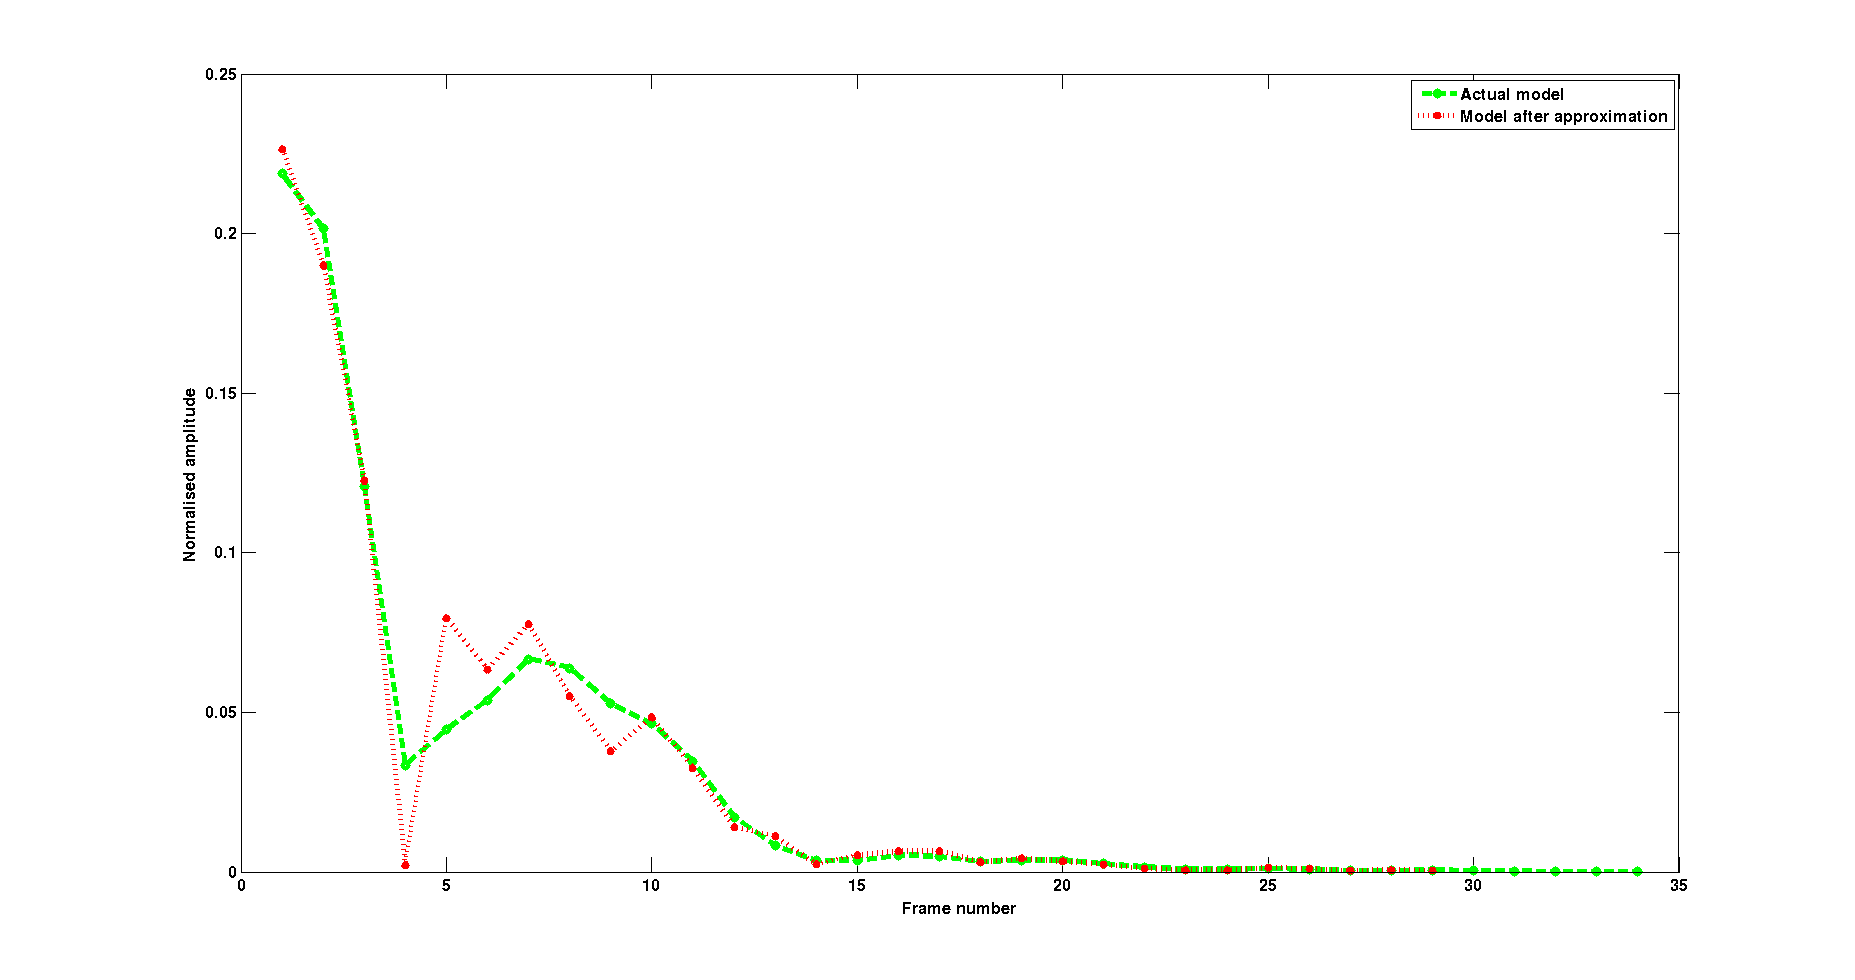
\includegraphics[width=9cm, height=6cm]{narrow_band_RIR_model}
\caption{Comparison of estimate of H with the actual H for k fixed at 50}
\label{fig:compare_true_expected}
\end{figure}

We compare the estimated $\mat{H}$ obtained using the reference approaches (N-CTF and N-CTF+NMF) to the
$\tilde{\mat{H}}$ for a RIR of $T_{60}$ approximately $700$~ms. These narrow band estimate of RIR obtained by reference methods with the actual value is plotted in Fig.~\ref{fig:compare_RIR_NMF}. It can be seen that the estimated RIR matches the expected RIR more closely during the later part of the RIR.  In the early part of the RIRs, the estimates are more erroneous, when compared to
the later parts. This is one of the main motivations for the proposed approach,
where we intend to use appropriate regularizer on $\mat{H}$ in the NMF approach
so that the estimated $\mat{H}$ is improved. Such an improved estimate for RIR,
will also lead to a better estimate of the speech signal leading to improved
speech enhancement and automatic speech recognition measures.
\begin{figure}
\centering
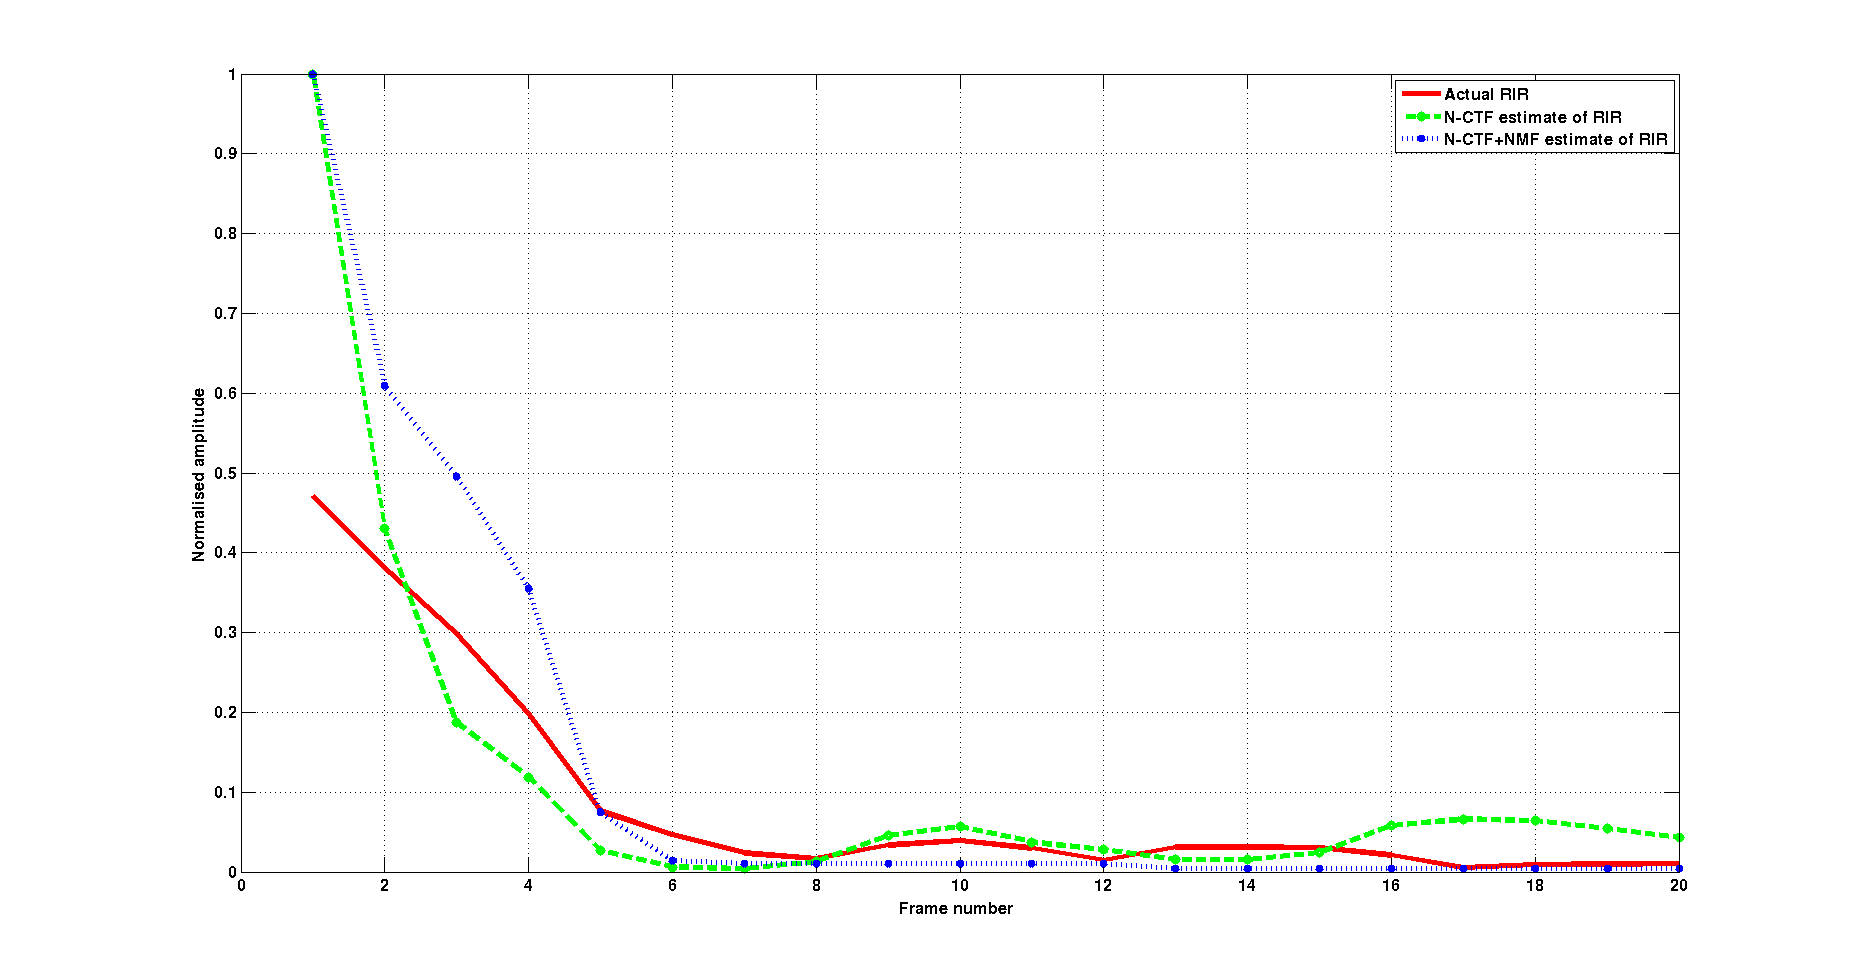
\includegraphics[width=9cm, height=6cm]{narrow_band_RIR}
\caption{Comparison of estimate of H with the actual H for k fixed at 50}
\label{fig:compare_RIR_NMF}
\end{figure}

% justification of early/late reflection effects in the reverberated speech signal
% XXX mention about regularizer used in multi-channel case
We propose three possible regularizations to the $\mat{H}$ for obtaining better
estimates of $\mat{H}$. We discuss the three choices and the corresponding cost
function.
\subsection{Sparsity of RIR}
\label{ssec:sparse_RIR}
Characterising RIRs of a reverberant room is challenging, as the RIRs depends on the room characteristics and distance between the source and the microphone acquiring the signal. However, the time-domain model by Pollack is a reasonable
characterisation based on the $T_{60}$ of a room model. Similarly, the
frequency-domain characterisation by Schroder is also a good model that has been
used extensively \cite{naylor2010speech}. It does not provide a characterisation of the
frequency-response but provides a characterisation of the possible distribution
of power with respect to frequency. In time-domain the RIR is exponentially
decaying with the decay factor dependent on the $T_{60}$. Correspondingly the
frequency domain representation of the RIR also has larger magnitude values
during the early part of the reverberation and the magnitude spectrum dies down
to smaller values during the late part. Most of the entries in H has a value very close to zero. Hence the simplest constraint is to
assume that the $\mat{H}$ has a sparse structure. This is different from
assuming sparsity on the speech signal. Assuming sparsity on $\mat{H}$ is
similar to assuming a sparse basis vector matrix in the standard NMF domain. We incorporate this into the basic NMD framework and have the modified
cost-function,
\begin{align}
  J(\mat{W}, \mat{X},\mat{H}) &= D_{KL}\left(\mat{Y}, \mat{X}\right),\\
  &= D_{LS}\left(\mat{Y}, \sum_{m} \mat{H}_m \stackrel{m\rightarrow}{\mat{S}}\right)
  + \lambda \parallel \mat{H} \parallel_1 \\
  \text{s.t.} & \mat{H}_m \ge 0, \mat{S} \ge 0.
  \label{eqn:NMFD_NMFcost_prop1}
\end{align}
$\lambda$ decides the weight given to sparsity of H. In the work, $\lambda = 1$. This method is referred to as N-CTF+Sparse H.
\subsection{Sub-band gains constrained RIR}
\label{ssec:gain_RIR}
Depending on the $T_{60}$ of the room and the distance between the source and
microphone the sub-band gain in the RIRs can be modelled as a function of the
frequency $Gain[k]$. Such models can be obtained by fitting
polynomial functions on existing recorded RIRs and their STFTs. This can be
included in the NMD framework as opposed to constraining the sub-band sums of
$\mat{H}$ to be unity. The corresponding cost function is,   
\begin{align}
  J(\mat{S},\mat{H}) &= D_{KL}(\mat{Y}, \mat{X}),\\
  &= D_{KL}\left(\mat{Y}, \sum_{m} \mat{H}_m
  \stackrel{m\rightarrow}{\mat{S}}\right) \\
  \text{s.t.} \sum_m H[k,m] = Gain[k],\ & k\in\{0,1,...,K-1\}\\
  \mat{H}_m \ge 0, \mat{S} \ge 0
  \label{eqn:NMFD_NMFcost_prop2}
\end{align}
where the $Gain[k]$ is to be obtained from existing RIRs or RIR models. This model is referred to as N-CTF+Gain H. 

\subsection{Inclusion of early part of RIR}\label{ssec:Hear_RIR}
RIR can be broadly divided into two regions - early reverberation and reverberation tale (late reverberation). The early part accounts for the reflections which come up to 50ms after the direct path. The reflections which come after 50 ms forms the reverberation tale. A sample RIR is shown in the fig. \ref{fig:RIR_plot}. The early part modifies the spectrum within a phone region, whereas the late reverberation results in changing the spectral characteristics of the present phone by the preceding phone. It is shown in the literature that late reverberation causes degradation of speech and need to be removed. However, retaining the early part improves speech intelligibility and ASR performance \cite{naylor2010speech}\cite{delcroix2014linear}. Once the clean 
speech spectrum ($S$) is estimated, the early part of RIR ($H_{ear}$) is attached to it using the following equation to obtain an improved dereverberated spectrum ($S_{new}$). 
\begin{figure}
\centering
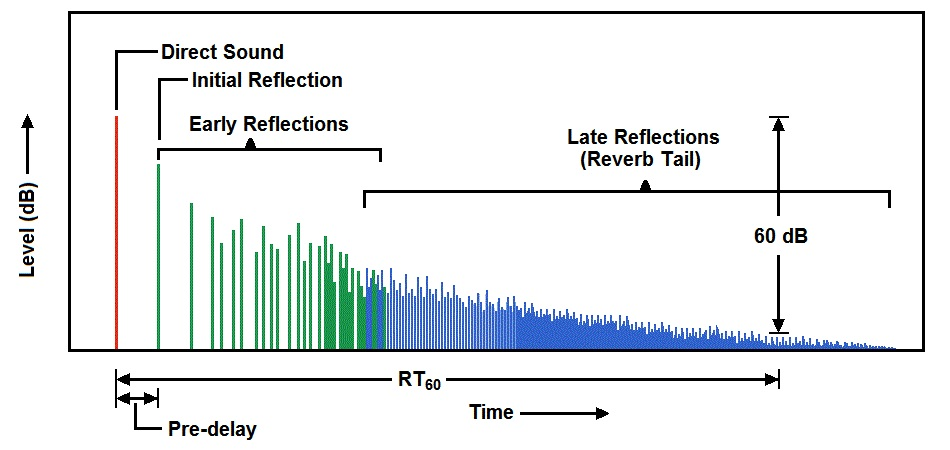
\includegraphics[width=8cm, height=6cm]{reverberation2}
\caption{Time domain representation of a typical RIR~\cite{rir_plot}}
\label{fig:RIR_plot}

\end{figure}
\begin{equation}
S_{new}(n,k) = S(n,k)*H_{early}(n,k), k\in\{0,1,...,K\}
\end{equation}
This method is referred to as N-CTF+$H_{ear}$. The algorithm using both N-CTF+$H_{ear}$ and N-CTF+Gain H is refereed to as N-CTF+$H_{ear}$+Gain H.
%\section{Formatting your paper}
%\label{sec:format}
%
%All printed material, including text, illustrations, and charts, must be kept
%within a print area of 7 inches (178 mm) wide by 9 inches (229 mm) high. Do
%not write or print anything outside the print area. The top margin must be 1
%inch (25 mm), except for the title page, and the left margin must be 0.75 inch
%(19 mm).  All {\it text} must be in a two-column format. Columns are to be 3.39
%inches (86 mm) wide, with a 0.24 inch (6 mm) space between them. Text must be
%fully justified.

\section{Results}
The performance of the algorithms discussed in section~\ref{prop_method} are evaluated for both speech enhancement and automatic speech recognition tasks (ASR).
\subsection{Database}
Two databases (TIMIT and TIDIGITS) have been used for the experiments. TIMIT contains two sets of data (train and test). Train set contains 10 sentences spoken by 377 different speakers and test set contains 10 sentences spoken by 168 distinct speakers. There are no common speakers in test and train sets. Out of the 10 sentences, 2 Sentences is common across all speakers. The performance in speech enhancement task is compared using a subset of TIMIT database. A set of 16 different sentences spoken by 16 distinct speakers is used. TIDIGITS contains 112 distinct adult speakers (55 male and 57 female) in train set and 113 different adult speakers (56 male and 57 female) in the test set. Each speaker has 77 utterances.  The database contains 11 distinct words (zero to nine and oh). The ASR performance is evaluated using adult data set of TIDIGITS. 

The word error rate (WER) of TIMIT database is relatively high ($\approx28\%$) for clean speech. Since the best achievable WER is itself high, a reliable WER improvement of various dereverberation algorithms cannot be analyzed using the database. The relative improvement in objective measures for the reference method using TIMIT database is available in \cite{mohammadiha2016speech}. To verify the implementation of reference method, TIMIT database is used for speech enhancement task. TIDIGITS is a limited vocabulary database with very low WER ($\approx1.5\%$). So TIDIGITS is used for comparing the performance of various algorithms for ASR task.   
\subsection{Evaluation measures}
The improvement in speech enhancement task is compared using improvement in three objective measures - perceptual evaluation of speech quality (PESQ), cepstral distance (CD) and speech-to-reverberation modulation energy ratio  (SRMR) \cite{falk2010non} \cite{reverb2014}. Dereverberated speech increases PESQ and SRMR score while CD tend to decrease as compared to reverberated speech. The effectiveness of the dereverberation algorithms is compared using the relative change in the objective measures of dereverberated speech ($\Delta PESQ$, $\Delta CD$ and $\Delta SRMR$) as compared with the reverberated speech.

Speech recognition performance is compared using the improvement in word error rate (WER) as compared to the reverberated speech. Speech recognition is performed using Kaldi toolkit trained on TIDIGITS. The speech recognition system has three sources of error - insertion, deletion, and substitution. For this task, the WER is defined as the ratio of the total number of misclassified phones to the total number of phones in the test set. Mathematically,
\begin{equation}
WER = \dfrac{INS + DEL + SUB}{Total\ number\ of\ phones\ in\ test\ set}*100\%
\end{equation}
where $INS$, $DEL$, $SUB$ represents the total number of insertion, deletion and substitution errors while decoding in the test set respectively. 
\subsection{Reference methods}
Two dereverberation algorithms NCTF and NCTF with speech model \cite{mohammadiha2016speech} are used as reference methods for comparison. In the reference paper, the objective measures PESQ, and CD were used for verifying the performance of the algorithm. The algorithm was tested on reverberated data generated using $16$ different TIMIT sentences which are spoken by $16$ distinct speakers. Reverberation is simulated using a measured RIR having a $T_{60}$ of around $680$~ms and DRR of $0$~dB was used. The NCTF model showed an improvement of about $0.3$ in PESQ score and $0.5$ in CD as compared to reverberated speech. The NCTF with speech model showed an improvement of $0.4$ in PESQ score and $0.4$ CD as compared to reverberated speech. The implementation of this method is verified by trying to reproduce the results in \cite{mohammadiha2016speech}. Although the exact RIR and set of sentences used in the experiments are unknown, we chose an RIR which has a $T_{60}$ and DRR of roughly $700$~ms and $0$~dB. Also, a subset of $16$ sentences spoken by different speakers from TIMIT database was used for performance evaluation. A PESQ score improvement of $0.46$ and CD improvement of $0.08$ is obtained for N-CTF method. Also, for N-CTF with speech model, a PESQ and CD improvement of $0.65$ and $0.1$ were obtained. The improvement obtained in PESQ score is comparable with the score obtained in \cite{mohammadiha2016speech}. However, improvements in CD was not comparable with the reference paper. The difference in obtained objective measure scores with the reference paper could be because of the different RIR and set of sentences used in the experiments. The implemented of algorithms are tested for other RIRs. Table \ref{tab:comparison_enhancement} shows the objective measure improvement for a different set of RIRs. Both PESQ and CD improves significantly improved for the reference methods. 
\subsection{Experiment setup}
The magnitude spectrogram is obtained using a $64$~ms window with a hop size of $16$~ms. The square root of Hanning window is used in analysis and synthesis side. The magnitude spectrogram of RIR (H) is represented using 20 frames. Out of which the first $2$ frames is related to the combination of direct path and early reverberation. H for each narrowband is initialized as a linearly decreasing function. S is initialized as the spectrogram of reverberated speech. For models with speech model, initial values for the basis and the activations are obtained by performing NMF decomposition on the spectrogram of reverberated speech. Since the algorithms converge fast, 20 iterations are performed for each algorithm to obtain the estimates of S and H.

Measured RIRs available from REVERB challenge \cite{reverb2014} is used for the evaluation. The RIRs are measured using an $8$ channel circular array of diameter $10$~cm. The RIRs of three rooms (small, medium and large) with $T_{60}$ of $250$~ms, $500$~ms and $700$~ms are available. The recordings are done for a microphone array placed $0.5$~m and $2$~m away from the source. 
The particular RIRs used for the experiment were measured in a room having a $T_{60}$ of $700$~ms with the microphone array placed $2$~m distant from the source. A similar trend in the dereverberation performance was observed for other RIRs. The dereverberation algorithms are performed by treating the 8 channel reverberated data as 8 independent recordings. 
\subsection{Speech enhancement for the proposed methods}
The performance of proposed dereverberation algorithms is compared using different objective measures. Since the microphones are placed very close to each other, the relative improvement in objective measures obtained across 8 channels is very close to each other. The net enhancement in the performance of different algorithms is obtained as an average of improvement in the objective measures for 16 sentences across 8 channels. The average objective measure improvement for various algorithms is shown in the Table \ref{tab:comparison_enhancement}.

From Table \ref{tab:comparison_enhancement}, it is observed that the baseline dereverberation algorithms N-CTF and N-CTF+NMF are able to enhance the reverberated speech.  Inducing sparsity (N-CTF+Sparse H) and frequency envelope on H (N-CTF+Gain H) does not improve the performance. 
The reason for the sparse H showing no improvement could be that narrow band H roughly has the exponentially decaying structure which we hope to achieve. 
The multiplicative update for the cost function in \eqref{eqn:NMFD_NMFcost_prop2} is obtained such that it minimizes the error in each narrowband independently. 
So the in effect cost function remains the same even after putting frequency envelope in H. 
All the objective measures show improvement for N-CNMF+$H_{early}$. However,  for N-CNMF+NMF+$H_{early}$, SRMR shows a significant improvement while other measures remain unchanged. The possible explanation can be that the algorithm reduces reverberation but also  adds distortion to the dereverberated speech. 
\begin{table}[th]
        \caption{\label{tab:comparison_enhancement} {\it The improvement in objective measures
        obtained using the proposed regularization to the RIR are compared with
      existing NMF based approaches.}}
        \vspace{2mm}
        \centerline{
          \begin{tabular}{|l|c|c|c|} \hline
            Methods & $\Delta PESQ$ & $\Delta CD$ & $\Delta SRMR$ \\ \hline \hline         
            N-CTF & $0.286$ & $0.671$& $1.200$\\
            N-CTF + $\mat{H_{early}}$ & $0.356$ & $0.722$& $1.611$\\
            N-CTF + Gain $\mat{H}$ & $0.278$ & $0.659$& $1.008$\\
            N-CTF + $\mat{H_{early}}$ + Gain $\mat{H}$ & $0.364$ & $0.718$& $1.557$\\
            N-CTF + Sparse $\mat{H}$ & $0.286$& $0.671$& $1.200$\\
            N-CTF + NMF speech & $0.570$& $0.909$& $1.236$\\
            N-CTF + NMF speech + $\mat{H_{early}}$ & $0.525$& $0.914$& $1.883$\\            
            \hline
          \end{tabular}
       }
\end{table}
\subsection{ASR improvement for the proposed methods}

The speech recognition system using Kaldi toolkit was trained using a Gaussian mixture model (GMM) - hidden Markov model (HMM) system. The system was trained using training data set of TIDIGITS. It contains 56 male and 58 female speakers speaking 77 utterances each. The GMM is an 8 Gaussian mixture. The HMM is a monophone with 1000 tied states. The ASR results obtained for an RIR with $T_{60}$ of $700$~ms and $2$~m away from the source is shown in Table \ref{tab:comparison_asr}.

The N-CTF model shows significant improvement in WER.  
N-CTF+Sparse H and N-CTF+Gain H methods show no improved the performance.
N-CTF+$H_{early}$ shows marginal improvement.
Methods including speech model (N-CTF+NMF and N-CTF+NMF+$H_{early}$) also show marginal improvement over N-CTF even though the objective measures shown significant improvement. The reason could be that dereverberation using speech model induced artifacts which do not affect the enhancement but affected the ASR performance. 
This can be observed in the estimate of H which shows distortions whereas for the N-CTF, the H estimate is smooth. N-CTF+NMF+$H_{early}$ has no significant improvement in ASR results as compared to N-CTF+NMF. 
\begin{table}[th]
        \caption{\label{tab:comparison_asr} {\it The improvement
        obtained for ASR task using the proposed regularization to the RIR are compared with
      existing NMF based approaches.}}
        \vspace{2mm}
        \centerline{
          \begin{tabular}{|l|c|c|} \hline
            Methods & $WER(\%)$ & $\Delta WER (\%)$  \\ \hline \hline  
            Clean speech & $1.76$ & $-$\\
            Reverberated speech &$29.03$ & $-$\\      
            N-CTF & $19.97$ & $9.06$\\
            N-CTF + $\mat{H_{early}}$ & $19.26$ & $9.77$\\
            N-CTF + Gain $\mat{H}$ & $20.06$ & $8.97$\\
            N-CTF + $\mat{H_{early}}$ + Gain $\mat{H}$ & $19.61$ & $9.42$\\
            N-CTF + Sparse $\mat{H}$ & $19.50$& $9.53$\\
            N-CTF + NMF speech & $19.24$& $9.79$\\
            N-CTF + NMF speech + $\mat{H_{early}}$ & $19.21$& $9.82$\\            
            \hline
          \end{tabular}
       }
\end{table}
\subsection{ASR improvement on beamformed output}
This section discusses the ASR performance a 2 stage dereverberation system. In the first stage, beamforming is performed using BeamformIt toolkit \cite{anguera2007acoustic} to obtain an enhanced single channel data obtained from 8 channel data. The second stage is a single channel dereverberation methods using the proposed methods. The second stage reduces the residual reverberation present after beamforming. The reverberation conditions and training set are same as in earlier experiments, but testing is done in a reduced set of 6 speakers (3 males and 3 females).

Table \ref{tab:comparison_asr_red1} shows the ASR performance of dereverberation using beamforming and proposed methods. The reference method N-CTF shows improvement in WER as compared with the beamformed output. This shows that the algorithm is able to suppress the residual reverberation present in the channel after beamforming. Other proposed algorithms failed to improve the WER any further. Table \ref{tab:comparison_asr_red2} compares the performance of proposed methods for the beamformed output in the presence of reverberation and noise. The algorithms perform poorly. The reason could be that the algorithm is designed to model reverberation alone. So in the presence of residual noise after beamforming, the algorithm fails to produce a good estimate of clean speech.  
\begin{table}[th]
        \caption{\label{tab:comparison_asr_red1} {\it The improvement in reverb speech ASR
        obtained using the beamforing followed by proposed methods.}}
        \vspace{2mm}
        \centerline{
          \begin{tabular}{|l|c|c|} \hline
            Methods & $WER(\%)$ & $\Delta WER (\%)$  \\ \hline \hline  
            Clean speech & $1.32$ & $-$\\
            Reverberated speech &$27.15$ & $-$\\  
            Beamforming & $22.2$ &$4.96$\\    
            N-CTF & $16.34$ & $10.82$\\
            N-CTF + $\mat{H_{early}}$ & $16.47$ & $10.69$\\
            N-CTF + NMF speech & $16.6$& $10.56$\\
            N-CTF + NMF speech + $\mat{H_{early}}$ & $17.33$& $9.83$\\            
            \hline
          \end{tabular}
       }
\end{table}
\begin{table}[th]
        \caption{\label{tab:comparison_asr_red2} {\it The improvement in reverb+noise(10dB) speech ASR
        obtained using the beamfoming followed by proposed methods.}}
        \vspace{2mm}
        \centerline{
          \begin{tabular}{|l|c|c|} \hline
            Methods & $WER(\%)$ & $\Delta WER (\%)$  \\ \hline \hline  
            Clean speech & $1.32$ & $-$\\
            Reverberated speech &$56.19$ & $-$\\  
            Beamforming & $41.63$ &$17.88$\\    
            N-CTF & $77.93$ & $-18.42$\\
            N-CTF + $\mat{H_{early}}$ & $77.87$ & $-18.36$\\
            N-CTF + NMF speech & $73.06$& $-13.55$\\
            N-CTF + NMF speech + $\mat{H_{early}}$ & $53.69$& $5.82$\\            
            \hline
          \end{tabular}
       }
\end{table}
\section{Conclusions and future work}
 The speech enhancement and ASR performance of speech dereverberation algorithms for various constraints on RIR are studied. 
The addition of sparsity and frequency envelope of RIR does not change the speech enhancement performance of the algorithm as compared with the baseline N-CTF model. But the inclusion of early part of RIR ($H_{early}$) with the estimate of clean speech improved the objective measures. The objective measures for reference method with speech model (N-CTF+NMF) also showed  improvement when $H_{early}$ was included in the model. 

The dereverberation using C-NMF reduced significantly the ASR performance. The inclusion of sparsity and frequency envelope did not change the WER. $N-CTF+H_{early}$ method shows a marginal improvement in ASR performance.  The inclusion of speech model ($N-CTF+NMF$) also did not show significant improvement in ASR performance. However, the algorithms were able to residual reverberation present in a beamformed output, but the algorithm fails to improve the performance in the presence of background noise. 
 
The dereverberation algorithms are not able to completely remove the effects of reverberation. A better model for reverberation and speech could improve the performance of dereverberation algorithm. Replacing NMF model for the clean speech by a convolutive NMF model could be one such approach. The use of multichannel data helps in dereverberation \cite{naylor2010speech}. The proposed methods can be modified to handle multichannel data. Also, other multichannel dereverberation algorithms like beamforming have to be studied. The effects of noise in distance speech recording are unavoidable. The performance of dereverberation algorithms is affected by the presence of noise. The proposed methods perform poorly in the presence of noise as discussed in section. So there is a need for modifying the proposed models to include the effects of noise. Other methods which perform dereverberation and denoising together should also need to be studied.  

\fi